%% ------------------------------------------------------------------
%%	Preamble start
%% ------------------------------------------------------------------
% Dokumentklassen
\documentclass[a4paper,danish,8pt,oneside,openany]{memoir}

% Definering af margin
\usepackage[left=4cm,right=4cm,top=6cm,bottom=6cm]{geometry}

%Så der ikke står kapitel x før egen chapter titel.
\chapterstyle{section}

%Dybde på nummeringen af sektioner.
\setsecnumdepth{subsection}

% Dybde på TOC
\settocdepth{subsection}

% Dansksproget dokument med dansk orddeling
\usepackage[danish,english]{babel}														

% Tegnsættet; utf8, ansinew, latin1
\usepackage[utf8]{inputenc}															

% Europæiske fonte
\usepackage[T1]{fontenc}																

%Matematik
\usepackage{amsmath, amssymb}

%Mere matematik.
\usepackage{mathtools}										

%Viser kun formelreferencer ved henvisninger.
\mathtoolsset{showonlyrefs}

% Pæne rules i tabeller
\usepackage{booktabs}

% Hyperlinks i pdf
\usepackage{hyperref}
\hypersetup{
    colorlinks,
    citecolor=black,
    filecolor=black,
    linkcolor=black,
    urlcolor=black
}

\usepackage{graphicx}


%% ------------------------------------------------------------------
%%	Dokument titel m.m.
%% ------------------------------------------------------------------
\title{Datamining report \\ Databaser og datmining 2015}
\author{Jonathan Schrøder Holm Hansen // fdg890}
\date{\today}

% Side layout, plain er kun side nummer. 
\pagestyle{plain}

%% ------------------------------------------------------------------
%%	Preamble slut
%% ------------------------------------------------------------------
\begin{document}	% Dokument start
\selectlanguage{english} % Hvis man bruger flere sprog i sit dokument. Refererer til babel.

\begin{titlingpage}
\maketitle
\end{titlingpage}
\section*{Preliminary comments}
This report is part of the solution to the final assignment for the datamining part of the course $Databases \ and \ datamining$ at DIKU, spring 2015.
%
The report presents the accomplished results, interprets when necessary, and introduces some thoughts on the chosen ways to solve the assignment.
Solutions were computed using Python 3.4 and SQLite3. The entire deliverable consists of:
%
\begin{itemize}
\item This final report
\item The Python scripts used to solve the assigned problems
\item Command prompt prints of the compiled script in .txt
\item README.txt listing used tools and programs
\end{itemize}
%
\vspace*{0.3cm}
%
\section*{Photometric Redshift Estimation}
\subsubsection*{1.2 Mean and sample variance}
%
The sample mean of $Redshift\_Train\_Y$ was calculated using the library average function of SQLite3. This solution seemed straight forward and had only the disadvantage that the sample mean was not stored in a variable.
\\
\\
The biased sample variance of $Redshift\_Train\_Y$ was found in the same way as the sample mean using extended relational algebra statements in SQLite3. The choice to solve the problem without storing the sample mean in a variable forced me to copy it from print to the SQLite3 statement, which may in theory pose a possible loss of precision due to rounding of the printed sample mean. However the used data set holds three decimals so I decided that my computed 16-decimal solutions was sufficiently precise (se the command promt script). The sample mean and the biased sample variance are reported in figure 0.1.
\\
\begin{figure}[!h]
\centering
\begin{tabular}{|r|r|}
\hline
\textbf{Sample mean} & \textbf{Biased sample variance}\\ \hline
0.1555464 & 0.0136722 \\ \hline
\end{tabular}
\caption{Data: Redshift\_Train\_Y}
\end{figure}
\newpage
%
\subsubsection*{1.3 Linear regression}
Building the affine linear model for $Redshift\_Train$ required calculations that was impossible (or at least very difficult) in relational algebra why the data was imported to matrices using a simple for loop that reads one row of a data table at a time. With the data in matrices the package $numpy$ (also used to create the matrices) enabled computation of the model parameters. First however a column of 1s was added to the $Redshift\_Train\_X$-matrice. The model parameters are reported in figure 0.2.
\\
\begin{figure}[!h]
\centering
\begin{tabular}{|l|r|}
\hline
 & \textbf{Model parameters}\\ \hline
$w_1$ & -0.00598922 \\ \hline
$w_2$ & 0.10965194 \\ \hline
$w_3$ & 0.27844859 \\ \hline
$w_4$ & -0.00183018 \\ \hline
$w_5$ & 0.00935054 \\ \hline
$vw_6$ & -0.00863705 \\ \hline
$w_7$ & 0.00414825 \\ \hline
$w_8$ & -0.10749617 \\ \hline
$w_9$ & -0.0098086 \\ \hline
$w_10$ & 0.04078572 \\ \hline
$w_11$ & -0.88069336 \\ \hline
\end{tabular}
\caption{Data: Redshift\_Train}
\end{figure}
\\
\\
The training error of the model could be found by computing the mean-squared error (MSE) of the model over $Redshift\_Train$. First the sum-of-squares error, J, was computed using a for loop that proceeded row by row through tables $X$ and $Y$. The result was divided by the number of elements in the set - 2500 in this case. The MSE is reported in figure 0.3.
\\
\begin{figure}[!h]
\centering
\begin{tabular}{|c|}
\hline
\textbf{Mean-squared error, MSE} \\ \hline
0.00280929 \\ \hline
\end{tabular}
\caption{Data: Redshift\_Train}
\end{figure}
\\
\\
Figure 0.4 shows the MSE of $Redshift\_Train$ next to the biased sample variance. The MSE is significantly (informally (possibly formally as well)) lower than the biased sample varience. First of all this suggests that a linear model is justified. Our estimated dependent variables are closer to the actual data than there is variance within the data. However this also means that there is some variance in the dependent variables that our model does not capture. In other words our model parameters predicts dependant variables that on an average are closer to the regression line that it is actually the case. One reason for this could be that there is some randomness in the data or that some significant information is not captured by the data variables.
\\
\begin{figure}[!h]
\centering
\begin{tabular}{|r|r|}
\hline
\textbf{MSE} & \textbf{Biased sample variance}\\ \hline
0.00280929 & 0.0136722 \\ \hline
\end{tabular}
\caption{Data: Redshift\_Train}
\end{figure}
\\
To find the test error of the model it was run over the $Redshift\_Test$ data. This means that the model parameters from the $Redshift\_Train$-model was tested over a so far unused set of data. Figure 0.5 shows the mean-squared error of the model build on $Redshift\_Train$ over $Redshift\_Test$ and the biased sample variance of $Redshift\_Test$:
\\
\begin{figure}[!h]
\centering
\begin{tabular}{|r|r|}
\hline
\textbf{MSE} & \textbf{Biased sample variance}\\ \hline
0.00319585 & 0.0147140 \\ \hline
\end{tabular}
\caption{Model: Redshift\_Train Data: Redshift\_Test}
\end{figure}
\\
The MSE is a little higher when our model is used over the $Test$ dataset. As it shows the biased sample variance is also a bit higher, which might account for some of the poorer performance of the model. Overall the model performs well. As before the MSE is lower than the biased sample variance when used on both datasets which is a good thing.
\newpage
%
%
\section*{Cyberfraud}
\subsubsection*{2.1 Classification}
The nearest neighbour classifier (1NN) was build on two helping functions. The first, $distance$, simply computes the distance between two vectors using the numpy.linalg-function $norm$ that gives the length of a vector.\\
\\
The second helping function, $minDistance$, takes a matrix and a vector representing a datapoint and finds the vector/datapoint in the matrix that is closest to the given vector. This function uses $distance$ and a for loop to run through the entire matrix.
\\
\\
The main function of the 1NN, $compareY$, uses $minDistance$ to go vector by vector through one matrix and finding the nearest vector in another matrix. While doing this $compareY$ also compares the dependent values of the two matrices and keeps count on the matches.\\
Finally the performance of the 1NN is translated to a percentage using simple calculations. The result is reported in figure 0.6:
\\
\begin{figure}[!h]
\centering
\begin{tabular}{|r|r|}
\hline
\textbf{Truecount} & \textbf{Performance}\\ \hline
157 & 98.125 \%  \\ \hline
\end{tabular}
\caption{Performance of 1NN}
\end{figure}
%
\subsubsection*{2.2 Dimensionality reduction and visualization}
To conduct a principal component analysis two functions were written. First however the covariance matrix of $Keystroke\_Train\_X$ was computed using the numpy.cov library function. Likewise the eigenvectors and eigenvalues were computed using numpy.eigh. For some peculiar reason the eigenvalues were listed in increasing order.\\
The first function written, $sumInc$, simply sums a specified number of values from a matrix from top down.
The model function, $PSA$, computes how many eigenvalues are needed to reach a desired level of explained variance. Results are reported below in figure 0.7.
\\
\begin{figure}[!h]
\centering
\begin{tabular}{|r|r|}
\hline
\textbf{Componentcount} & \textbf{Explained variance}\\ \hline
7 & 92.02 \%  \\ \hline
\end{tabular}
\caption{PCA analysis of components needed to reach 90\% explained variance}
\end{figure}
\\
The first of the following scatterplots shows the eigenvalues of the covariance matrix. Notice that the two principal components make up close to two thirds of the eigenvalue sum meaning that these two dimensions are vital in a dimension reduction.\\
The second scatterplot simply shows the data encoded to two dimensions.
\\
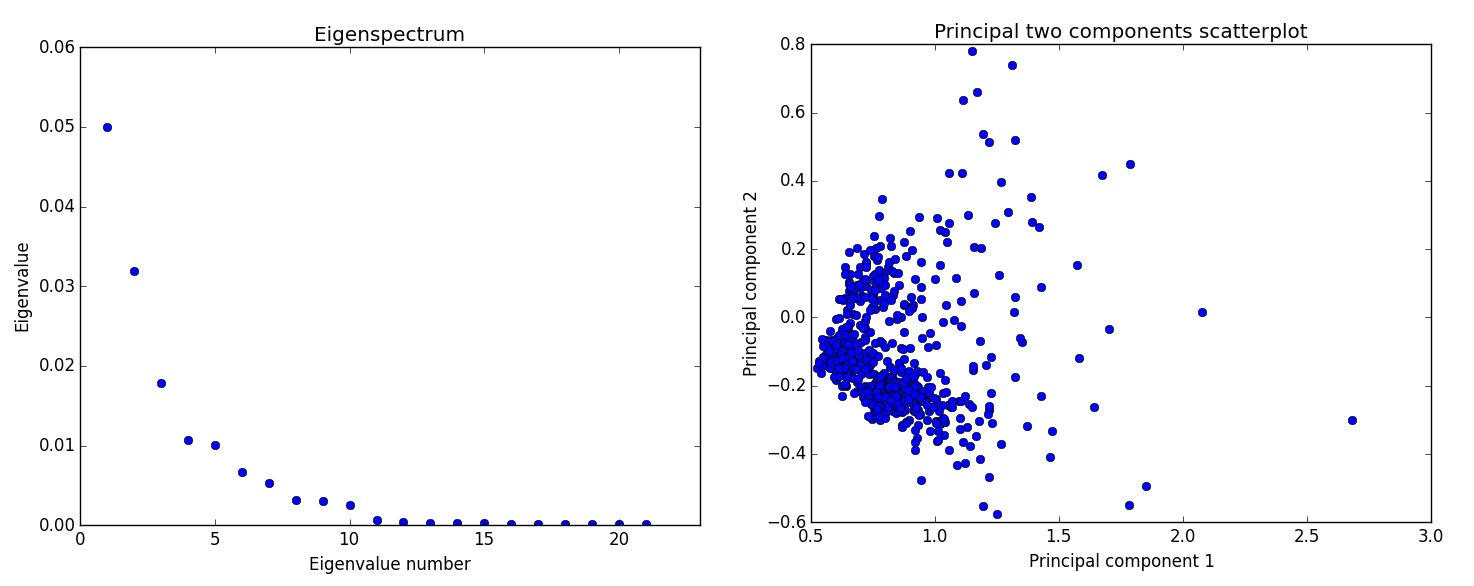
\includegraphics[scale=0.44]{Scattertimes2}
%
\subsubsection*{2.3 Clustering}
To conduct the 2-means clustering a few functions were written. The first, $clusterAssign$, assigns a datapoints to one of two clusters for an entire dataset.\\
The main clustering function, $twoMeansCluster$, repeatedly assigns datapoints to one of two clusters and computes new cluster centroids to assign by until the new centroids are the same as in the previous iteration.\
Finally a function, $clusterDistortion$, computes the distortion measure of the found clusters. Figure 0.8 shows the results.
\\
\begin{figure}[!h]
\centering
\begin{tabular}{|r|r|r|}
\hline
& \textbf{Cluster n} & \textbf{Distortion} \\ \hline
\textbf{Cluster 1} & 304 & 22.6\\ \hline
\textbf{Cluster 2} & 336 & 52.1\\ \hline
\end{tabular}
\caption{Results of 2-means clustering}
\end{figure}
\newpage
The following is a scatterplot of the cluster data base shifted using the two principal components. Judging by appearance the clusters are meaningful. The boundary between the clusters is a clearly visible line and only few datapoints seem to "out of place".
\\
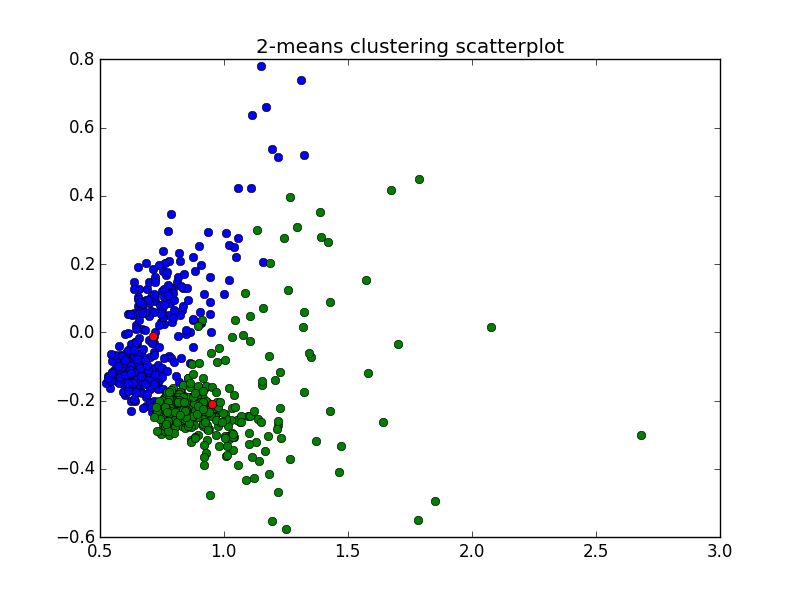
\includegraphics[scale=0.64]{2meansCluster}
\end{document}